\section{The Structured Adaptive Mesh Refinement (SAMR) Method}
\label{sec.amr}

%\subsubsection{SAMR Overview}

%Unlike moving mesh methods \citep{1995ApJS..100..269P,1995ApJS...97..231G} or  methods that subdivide individual cells \citep{Adjerid}, Berger \& Collela's AMR (also referred to as \emph{structured} AMR) utilizes an adaptive hierarchy of grid patches at varying levels of resolution.  The SAMR method described here is similar to \citet{Berger89}.  A more complete discussion of the history and development of this type of algorithm is available in \citet{Neeman96}.

The back-bone of the SAMR idea is the patch, or grid, which we take to be rectilinear to simplify bookkeeping (in practice, the lower-level routines such as the hydro solvers all assume Cartesian coordinates).  The single root grid covers the entire computational domain and plays the role of the root node in the grid hierarchy.  Subgrids are placed such that they cover (hopefully small) sub-volumes of the root grid at higher resolution.  This structure forms a tree that may be extended to arbitrary depths by adding additional grids to refine regions in the subgrids.  We use the following notation to describe grid relationships.  A grid's \textit{parent} is the coarse grid that completely contains it.  The \textit{root grid} is the most coarsely-resolved grid, and it has no parent.  A \textit{child grid} is a grid completely contained by its parent grid (note that a grid may have many children but only one parent), while sibling grids are those that have the same resolution, but not necessarily the same parent.  We also refer to levels of the hierarchy, where the root grid is labeled level zero and all grids with the same resolution are on the
same level.

In order to simplify bookeeping, a number of restrictions are imposed on the subgrids:
\begin{itemize}
 \item The refinement factor $r$, or the ratio of the coarse cell width to the fine cell width, must be an integer.  In practice, \enzo\ almost always uses $r=2$, since tests have shown this typically provides the best performance.
 \item Each subgrid must begin and end on the boundary of a coarse cell.  This means that the number of cells in a patch will be a multiple of the refinement factor.
 \item A subgrid must be completely enclosed by its parent.
\end{itemize}

The AMR grid patches are the primary data structure in \enzo.  Each patch is treated as an individual object that can contain both field variables and particle data.  Individual grids are organized into a  dynamic, distributed hierarchy of mesh patches.  
%See Figure~\ref{fig.2.amrhierdens} for an example of an \enzo\ simulation performed using this AMR scheme where both the baryon density and AMR grid hierarchy are shown together. 
% GB: I think this figure is too application-specific

\begin{figure}
\begin{center}
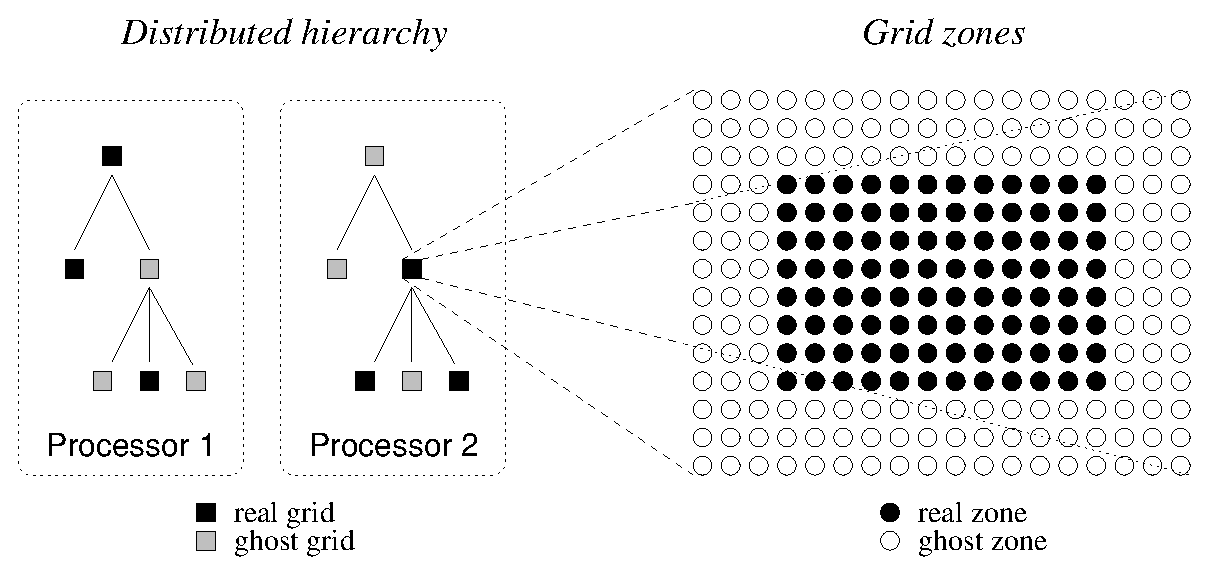
\includegraphics[width=0.5\textwidth]{figures/amr_hierarchy.eps}
\end{center}
\caption{\emph{Left:} Example of a simple, distributed AMR hierarchy
showing real and ghost grids.  \emph{Right:} Example 2D \enzo\ grid
showing real and ghost zones, as needed for the PPM hydro stencil. }
\label{fig.amr_hierarchy}
\end{figure}

Each grid patch in \enzo\ contains arrays of values for baryon and particle quantities.   Grids are partitioned into a core of \emph{active zones} and a surrounding layer of \emph{ghost zones}, as shown in Figure~\ref{fig.amr_hierarchy}.  The active zones store field values and ghost zones are used to temporarily store values that have been obtained directly from neighboring grids or interpolated from a parent grid.  These zones are necessary to accommodate the computational stencil of the (magneto)hydrodynamics solvers (Sections~\ref{sec.hydro.ppm} through~\ref{sec.hydro.zeus}) and the gravity solver (Section~\ref{sec.gravity}).  The PPM and Zeus hydro solvers require 3 layers of ghost zones,  and the gravity solver requires 6 (although only for the density and potential fields).  This can lead to significant memory and computational overhead, particularly for smaller grid patches at high levels of refinement.  

From the point of view of the hydro solver, each grid is solved as an independent computational fluid dynamics (CFD) problem, with Dirichlet boundary conditions stored in the ghost zones.  At the end of each timestep, cells on a given level fill ghost zones by interpolating from the parent and copying from neighbors on the same level.  Grids then correct the flux at the interface boundary between fine and coarse zones, and finally project their active zone data to the parent grid. 

Timesteps are determined on each level as described in Section~\ref{sec.timestepping}, and the hierarchy is advanced on
a level-by-level basis in a W-Cycle.    Beginning with the coarsest level, $l$, all grids on that level are advanced one
timestep.  Then, one timestep is taken on all grids at the next level of refinement, $l+1$, and so on until the finest level is resolved. The finest level is then advanced, using as many steps as it takes to reach the level immediately above.  The finest level is then synched to the level above it, which then proceeds forward in time one more step.  This is shown graphically in Figure~\ref{fig:wcycle}.

At the end of every timestep on every level, each grid updates its ghost zones by exchanging information with its neighboring grid patches (if any exist) and/or by interpolating from a parent grid.  In addition, cells are examined to see where refinement is required and the entire grid hierarchy is rebuilt at that level (including all more highly refined levels).  The timestepping and hierarchy advancement/rebuilding process described here is repeated recursively on every level to the specified maximum level of refinement in the simulation. 

The basic control algorithm looks very much like any used in a grid-based code of a single resolution, and can be written schematically as:
\begin{verbatim}
InitializeHierarchy
While (Time < StopTime)
   dt = ComputeTimeStep(0)
   EvolveLevel(0, dt)
   Time = Time + dt
   CheckForOutput(Time)
\end{verbatim}
The AMR control algorithm is contained within the recursive
EvolveLevel algorithm, which takes the level upon which to operate as an
argument.  This looks something like the following pseudo-code:
\begin{verbatim}
EvolveLevel(level)
   SetBoundaryValues
   while (Time < ParentTime)
      dt = ComputeTimeStep(level)
      SolveHydroEquations(dt)
      SolveOtherEquations(dt)
      Time = Time + dt
      SetBoundaryValues
      EvolveLevel(level+1, dt)
      FluxCorrection
      Projection
      RebuildHierarchy(level+1)
\end{verbatim}

Each function operates on all the grids on the given level.  In the following sections, we will address each of the major elements in turn.

\subsection{Setting the boundary values}
\label{sec:interpolation}

In order to solve the hydrodynamic equations on a patch, it is necessary to specify the boundary conditions on that patch.  There are two cases.  The first is that the boundary is external to the computational domain.  This occurs for all the boundaries of the root grid.  The second possibility is that the boundary is within the computational domain, which is true for most, but not all, subgrids.

In the first case, we allow for four types of boundary conditions
(represented here as being at $x=0$, with positive $x$ interior and
negative $x$ exterior to the domain):
\begin{enumerate}
  \item{\em Reflecting.} In this case, the boundary behaves like a mirror, with the solution on the boundary reflecting the solution in the computational domain ($q(-x) = q(+x)$) but with the velocity normal to the boundary reversed: $v_x(-x) = -v_x(+x)$.
  \item{\em Outflow.}  We approximate outflow boundary conditions by duplicating the solution at the edge of the computational domain: $q(-x) = q(0)$.
  \item{\em Inflow.} In this case, the boundary values are fixed by a pre-determined function ($q(-x) = q0(-x,t)$).  The code provides a simple way to set inflow values that are constant in both time and space over an entire face, or hooks are provided for special cases where the boundary must be time-varying.
  \item{\em Periodic.} The boundary solution is obtained from the other side of the grid: $q(-x) = q(x_{\rm{max}}-x)$.
\end{enumerate}

In the second case, the value must be either (1) interpolated from a parent or (2) copied from a sibling.  In practice, we solve this problem by first interpolating all boundaries from the grid's parent and then performing the sibling copy wherever possible, since these values will always be as good as, or superior to, interpolation.

We focus first on conserved, cell-centered quantities.  The interpolation function should be conservative in the sense that the mean over the interpolated quantity, in a given cell, must return the cell-centered value.  It should also be monotonic, so that new extrema are not introduced into a smoothly varying field.

In one dimension, such functions are well known; examples include
donor cell, Van Leer, and piecewise parabolic interpolation, which are
first-, second-, and third-order accurate respectively
\citep[e.g.,][]{Stone92a}.  However, we require fully
multi-dimensional interpolation functions, and so focus on
second-order schemes since they are tractable and relatively 
accurate\footnote{We could, in principle, build a multi-dimensional
  interpolator out of a one-dimensional interpolation function;
  however, at higher order, this would not necessarily satisfy our
  constraint regarding not introducing new extrema in interpolated quantities.}.  In Appendix~\ref{app:interpolation}, we
explicitly write down functions in one, two and three dimensions, but
here we discuss the general design considerations.

In two dimensions, it is relatively easy to build a linear, monotonic,
conservative function by requiring, first, that the function at the
center of the cell return the cell-centered quantity (and since it is
linear, this implies that an average over the cell will also be equal
to this value), and second, by treating the cell-diagonals as
one-dimensional Van Leer-type functions.  The reason to focus on the
cell diagonals is that for a linear function, the extrema will occur at the cell 
corners, which are in turn linked by the diagonals.  This process can be done in
two dimensions since there are three constraints (one at the center and one along
each diagonal), and three parameters in a two-dimensional linear
function.

In three dimensions this process breaks down since the number of
constraints (center + four diagonals = five) exceeds the number of
parameters (four).  One way to solve this problem would be to perform
a least-squares fit under the given constraints; however, this is
too computationally expensive.  Therefore, in Appendix~\ref{app:interpolation} we describe
a heuristic approach that satisfies four constaints analytically and
then adjusts the interpolation parameters in such a way as to satisfy the fifth.
While the result is not necessarily optimal, it does appear to perform
adequately in our tests.

%The same procedure can be used for face-centered quantities; however, for the velocity variable in zeus, we drop the extrema constraint.

\subsection{Solving the hydrodynamic equations on a grid}
\label{sec:solve_hydro}

Given the grid and its boundary conditions, the process of solving
equations~(\ref{eq:mass})--(\ref{eq:total_energy}) can be detached
from the rest of the SAMR technique, so that it is possible to
experiment with a number of different methods.  The restrictions are
that the method should be flux-conservative, or at least produce an
accurate estimate of the flux of conserved quantities at cell
interfaces.  This is required in the flux-correction step (see
\ref{sec:flux_correction}).  There is also the issue of centering,
which refers to the position of physical quantities within a cell (the
primary types are cell-centered, face-centered, and node-centered). 
%In this description we will employ the direct Eulerian version of the piecewise
%parabolic method \citep{1984JCoPh..54..174C,1995CoPhC..89..149B}, which
%assumes cell-centering for all quantities (actually they are
%cell-averages).  
%However, it is also possible to use other schemes,
%which employ different centering for different variables
%\citep[e.g.,][]{Stone92a}.  
The interpolation step, described in
Section~\ref{sec:interpolation}, must correctly interpolate with the
selected centering.

\subsection{Projection}
\label{sec:projection}

Since a refined region is simulated with (at least) two different resolutions (one fine and one coarse), it has two or
more ``solutions'' (i.e.~values of density, velocity, etc.) that represent the same volume of space.  This is one important aspect of the SAMR method -- some physical regions are represented by grids at multiple resolutions.  To
maintain consistency, the coarse grid quantities are updated with the finer values, using a volume-weighted average of the conserved quantities:
\begin{equation}
q^{\rm coarse} = r^{-d} \sum q^{\rm fine}_{i, j,k}
\end{equation}
where $r$ is the refinement factor, and the sum is over all fine cells that ``cover" the coarse cell. The exponent, $d$, refers to the weight of the average.  For cell-centered quantities, this is the dimensionality of the problem.  For face-centered quantities, this is one less than the dimensionality, and for edge-centered quantities this is one.


\subsection{Flux correction}
\label{sec:flux_correction}

One of the significant advantages of flux-conservative methods is, of course, their ability to maintain conserved quantities to machine precision.  Unfortunately, the projection step upsets this flux conservation since, at the boundary of a refined region, the coarse and fine cells on either side of the border are updated with different estimates of the flux across the boundary.  At one refinement level this comes from the coarse grid computation, and in the other from the fine grid solution.  Conservation can be restored by correcting all coarse cells that lie outside the boundary of a fine region
with the difference between the coarse and fine estimates of the flux
across the boundary:
\begin{equation}
  q^{\rm coarse} = \tilde{q}^{\rm coarse} - \Delta t \left( F^{\rm
      coarse} - \sum_{j,k} F^{\rm fine}_{j,k} \right)
\end{equation}
where $F$ is the flux of quantity $q_i$ in the $i$-direction through the cell interface.   We use $\tilde{q}$ to indicate the uncorrected quantity on the coarse grid and the sum is over the $r^{d-1}$ fine cell interfaces in the perpendicular dimensions that share a face with the coarse cell being corrected.  This correction is carried out for all coarse cells that share a face with a refined cell (and are not themselves covered with more refined cells).

\subsection{Hierarchy reconstruction}
\label{sec:hierarchy_reconstruction}

Since the addition of more highly refined grids is adaptive, the conditions for refinement must be specified. Many different criteria can be simultaneously specified for a given simulation, and these refinement criteria are discussed in more detail in the following section (Section~\ref{sec:refinement_criteria}).   Once all cells in a given grid that require additional refinement have been flagged, rectangular boundaries are determined that minimally encompass the flagged cells.  This is done using an iterative machine-vision technique, as described in \cite{Berger91}.

We first find the smallest region (or ``proto-subgrid") that covers all of the refined cells on a grid.  We compute an efficiency $\epsilon$ for this grid, defined as the ratio of flagged cells to total cells.  If this efficiency is sufficiently large (typically over 30\%), or if the grid is small enough, then we adopt the region as a new grid and move on to the next region (if any).  If the region is not acceptable, then we split it into two using the following algorithm.  First, we determine the longest dimension and compute the signature along that dimension.  The signature is found by summing the number of refined cells with the same index along the longest dimension.  Edges are typically indicated by inflection points in this signature, so we calculate the second derivative using a simple three-point finite difference estimator and look for the maximum in the second derivative, with ties going to the index closest to the center.  If no inflection points are found along the longest axis, the next-longest axis is searched.  If no inflection points are found, the longest axis is cut in half.  The original region is then split into two new regions, or proto-subgrids.  This process is then re-applied to each of the new regions.

This algorithm is not necessarily optimal, but experience shows it does a reasonable job of generating an efficient covering of the refined cells.  Note that some cells are unnecessarily refined with the SAMR approach, resulting in wasted resources (unlike in cell-splitting AMR schemes).  However, it has a number of advantages.  First, traditional grid-based hydro methods can be simply added with only minor modifications.  Second, it is easier to accommodate larger stencils (as in PPM, which requires three boundary zones), and third, it can be more efficient for some machines since there are more predictable and linear memory accesses, which more efficiently use a CPU's cache.


\subsection{Refinement criteria}
\label{sec:refinement_criteria}

In this section, we turn to the refinement criteria themselves.
Although generalized refinement criteria are available based on
estimators for the error, such as the Richardson method \citep{AtkinsonHan2004}, we have focused generally on methods that use physical estimators based on the assumption that the simulator has a specific quantity or quantities that indicate the need for refinement.  The flagging methods currently built into \enzo\ are:

\begin{enumerate}

\item{\em Slope.}  If the normalized slope $(q_{i+1} - q_{i-1})/ (2 q_i)$ of baryon quantities between adjacent cells is larger than a specified value (typically 0.3), then the cell is flagged.

\item{\em Baryon mass.}  This refinement criterion is designed to
  mimic a Lagrangian method in that it tries to keep a fixed mass
  resolution.  In this method, a cell is refined if the baryonic mass
  in the cell ($M_g = \rho\, (\Delta x)^d$) is larger than a specified value:
\begin{equation}
M_g > \rho_{\rm flag}\, (\Delta x_{\rm root})^d r^{\epsilon_l l},
\end{equation}
where $\rho_{\rm flag}$ is the equivalent density on the root grid
required for refinement, $\Delta x_{\rm root}$ is the root grid cell
spacing, $r$ is the refinement factor, $l$ is the level and
$\epsilon_l$ is a parameter that can be used to make the refinement
more aggressive ($\epsilon_l < 0$) or less aggressive ($\epsilon_l >
0$) than pure Lagrangian refinement --- in other words,
super-Lagrangian or sub-Lagrangian in refinement.

\item{\em Shocks.}  In this method, we identify and refine cells that contain shocks using the following criteria:
\begin{eqnarray}
%% (p_{i+1} - p_{i-1})/\min(p_{i+1}, p_{i-1}) & > & 0.33,  \nonumber \\
%% u_{i-1} - u_{i+1} & > & 0, \quad\text{and} \\
%% e_i / E_i & > & 0.1.  \nonumber
(p_{i+1} - p_{i-1})/\min(p_{i+1}, p_{i-1}) > 0.33,  \qquad
u_{i-1} - u_{i+1} > 0, \quad\text{and} \qquad
e_i / E_i > 0.1.  \nonumber
\end{eqnarray}
We note that the parameters $0.33$ and $0.1$ in the equations above were determined empirically, and can be modified by the user to refine more or less aggressively, as the situation warrants.

\item{\em Particle mass.}  This refinement criterion is precisely the same as the baryon mass criterion except that it uses the gridded (cloud-in-cell, or CIC) particle density.  In general, this criteria is used in cosmological simulations, and thus refines on dark matter and stellar density.

\item{\em Jeans length.}  Following \cite{Truelove98}, the code can be forced to refine the Jeans length by a fixed number of cells, or, more specifically, whenever the following criterion is not met:
\begin{equation}
\Delta x < \left( \frac{\pi k_B T}{N_J^2 G \rho \mh} \right)^{1/2},
\end{equation}
where $J_J$ is the required number of cells per Jeans length (4 by default).

\item{\em Cooling time.}  Often in cosmological simulations, cooling is a rapid process and we do not necessarily want to be limited by the cooling time.  However, in some cases it is desirable to resolve the cooling process, in which case we flag cells that have a cooling time shorter than their sound crossing time.  The cooling time is given by $t_{\rm cool} = 1.5 k_BT / (n\, \Lambda(T))$ and the sound crossing time is $t_{\rm cross} = \Delta x / c_s$, where $c_s$ is the sound speed.

\item{\em Must-refine particles.}  In order to allow for refinement in moving regions, it is possible to generate ``must-refine" particles that ensure local refinement of the 8 nearest cells to a specific level.  The particles feel gravitational forces and their trajectories are followed as for any other collisionless particle.  This feature can be used to ensure that a specific Lagrangian region stays refined to a specified level of resolution. 

\item{\em Shear.} As described in \citet{Kritsuk06}, turbulence calculations can be successfully modeled with AMR if the shear is used as a refinement parameter; in particular, refinement occurs when the finite difference version of the following inequality holds:
\begin{equation}
%\left(\frac{du}{dy}\right)^2 + \left(\frac{du}{dz}\right)^2 + 
%\left(\frac{dv}{dx}\right)^2 + \left(\frac{dv}{dz}\right)^2 + 
%\left(\frac{dw}{dx}\right)^2 + \left(\frac{dw}{dy}\right)^2 
\sum_i \sum_j \left( \frac{\partial v_i}{\partial x_j} \right)^2 -  \sum_i \left( \frac{\partial v_i}{\partial x_i} \right)^2
> \epsilon_s \frac{c_s^2}{\Delta x^2},
\end{equation}
where $\epsilon_s$ is a dimensionless parameter.

\item{\em Optical depth.} This refinement criterion, typically used for simulations using radiation transport, ensures that cells on the highest level of refinement have an \ion{H}{1} optical depth lower than unity.  The optical depth of a cell is estimated to be:
\begin{equation}
\tau = \sigma_{\rm HI} n_{\rm HI} \Delta x 
\end{equation}
where $\sigma_{\rm HI}$ is the neutral atomic hydrogen absorption
cross section, $n_{\rm HI}$ is the proper \ion{H}{1} number density,
and $\Delta x$ is the cell width (which is assumed to be the same along each axis).  If $\tau > 1$, the cell is refined
further, up to the maximum level of refinement.

\item{\em Resistive length.}  In a way similar to the Jeans length criterion described above, the code can be forced to locally resolve the resistive length scale by a minimum of a fixed number of cells.  This is done by ensuring that the resistive length scale, defined as
\begin{equation}
L_R = |B| / |\curl B|
\end{equation}
is always refined by at least N$_R$ cells locally (i.e.~we refine a given cell further if $L_R \leq N_R \Delta x$).  Note that \enzo\ does not actually solve the resistive MHD equations -- this is the ``characteristic'' local resistive length, rather than one calculated within the MHD solver.

\item{\em Must refine region.}  This refinement criterion is used to ensure that all cells in a given subvolume of the simulation are refined to {\it at least} some minimum level of refinement.  The subvolume is user-specified, and may evolve over time (e.g., to follow a structure of interest that is traveling through the simulation volume).

\item{\em Metallicity.}  This refinement criterion ensures that all cells with a metallicity (defined as $Z \equiv \rho_{Z} / \rho_{b} / 0.022$, where $\rho_{Z}$ is the density of metals in the cell, $\rho_{b}$ is the total baryon density (including metals), and 0.022 is the solar mass fraction of metals) above a user-defined value is refined to {\it at least} some minimum level of refinement. 

\end{enumerate}

Finally, it is also possible to specify a rectangular region that is statically refined to a certain level.  These static refined regions are in place throughout the simulation regardless of the grid quantities and can be used for testing purposes, or for multiply-zoomed initial conditions (in cosmology simulations, for example) that would not otherwise be refined.

%GB: The following section has now been worked into the main text above and, I think, can be removed.
%
%\subsection{Adaptive mesh refinement}\label{sec.ov.amr}
%\dcc{removed most of the notes.  Added intro blurb.  moved parallelism
%  stuff. Re-worded the bit on ghost zones.  Summary of 'grid as
%  independent update + syncing with neighbors and parents,' W-cycle. Added
%  sentence on subgrid creation.  Made timestepping its own subsection.}
%\red{Talk about reasonable refinement factors - which 
%ones are usable, etc?}

%The primary purpose of the \enzo\ code is its Adaptive Mesh Refinement
%capability, which allows it to reach extremely large dynamical ranges
%with limited computational resources, opening doors previously closed
%by finite memory and computational time. Unlike moving mesh methods
%\citep{1995ApJS..100..269P,1995ApJS...97..231G} or  
%methods that subdivide 
%individual cells \citep{Adjerid}, Berger \& Collela's AMR (also referred 
%to as \emph{structured} AMR) utilizes an adaptive hierarchy of grid 
%patches at varying levels of resolution.  Each rectangular grid patch 
%(referred to as a ``grid'') covers some region of space in its 
%\emph{parent grid} which requires higher resolution, and can itself 
%become the parent grid to an even more highly resolved \emph{child grid}. 
%ENZO's implementation of structured AMR places no restrictions on 
%the number of grids at a given level of refinement, or on the number of 
%levels of refinement.  However, owing to limited computational resources 
%it is practical to institute a maximum level of refinement $\Lmax$.  

%The \enzo\ implementation of AMR allows arbitrary integer ratios of parent and
%child grid resolution.  However, in practice 
%refinement factors (defined as the ratio of parent grid resolution to child grid resolution) 
%of two or four are typically used, with a refinement factor
%of two being most commonly used for cosmological simulations for reasons of
%efficiency. The ratio of
%box size to the maximum grid resolution of a given simulation is
%therefore $L/e = \Nroot \times 2^{\Lmax}$, where $\Nroot$ is the
%number of cells along one edge of the root grid, $\Lmax$ is the
%maximum level of refinement allowed, and L and e are the box size
%and grid resolution of the most highly refined region, respectively.

%The AMR grid patches are the primary data structure in \enzo.  Each
%patch is treated as an individual object which can contain both field
%variables and particle data.  Individual grids are organized into a 
%dynamic, distributed hierarchy of mesh patches.  
%See 
%Figure~\ref{fig.2.amrhierdens} for an example of an \enzo\
%simulation performed using this AMR scheme where both the baryon density
%and AMR grid hierarchy are shown together. 

%\begin{figure}
%\begin{center}
%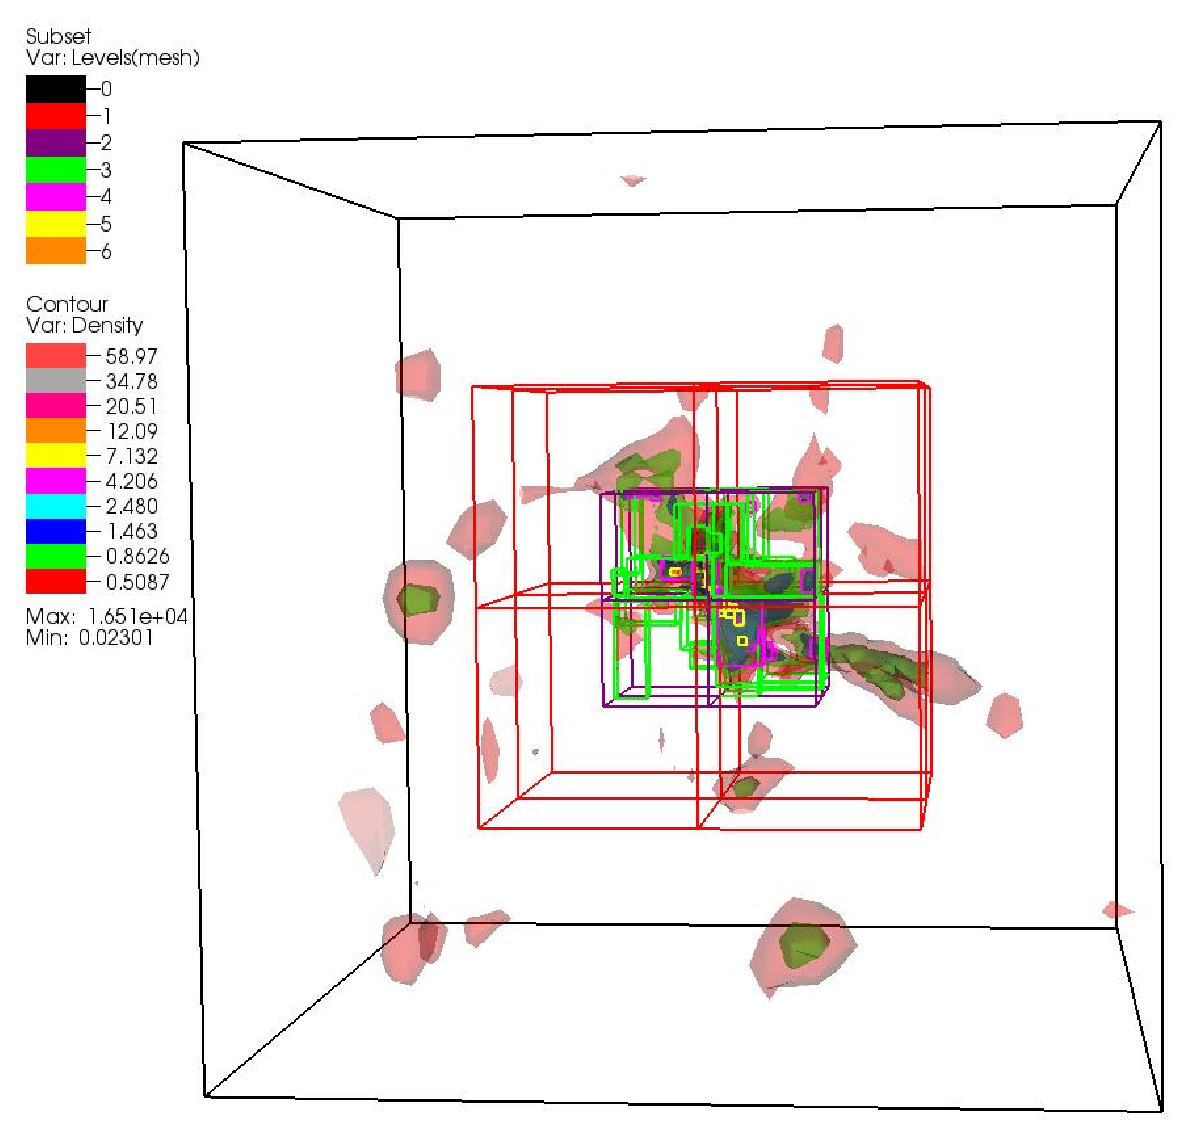
\includegraphics[width=0.4\textwidth]{figures/amr-hier-dens.eps}
%\caption{Example of an \enzo\ simulation showing the AMR grid hierarchy.  
%This is a simulation of the collapse of a single massive halo with a 
%$32^3$ root grid and two $32^3$ static nested grids.  AMR is only allowed
%within the most highly refined static nested grid.  Log baryon density is shown
%by colored isocontours with values corresponding to the legend at center left.  
%The rectangular solid wire frames correspond to individual 
%AMR grids, with different colors corresponding to level as indicated by the
%legend at top left.}
%\label{fig.2.amrhierdens}
%\end{center}
%\end{figure}

%Each grid patch in \enzo\ contains arrays of values for baryon and 
%particle quantities.   Grids are 
%partitioned into a core of \emph{real zones} and a surrounding layer 
%of \emph{ghost zones}.  The real zones store field values and ghost 
%zones are used to temporarily store values which have been obtained 
%directly from neighboring grids or interpolated from a parent grid.  
%These zones are necessary to accommodate the computational stencil of 
%the hydrodynamics solvers (Sections~\ref{sec.ov.hydro.ppm} and~\ref{sec.ov.hydro.zeus}) 
%and the gravity solver (Section~\ref{sec.ov.nbody}).  
%The PPM and Zeus hydro solvers require 3 layers of ghost zones,  and the gravity
%solver requires 6.  This can lead to significant memory 
%and computational overhead, particularly for smaller grid patches
%at high levels of refinement.  More information on filling of ghost
%zones can be found in the appendix.

%From the point of view of the hydro solver, each grid is solved as an
%independent CFD problem, with Dirichlet boundary conditions stored in
%the ghost zones.  At the end of each timestep, cells on a given level
%fill ghost zones by interpolating from the parent and copying from
%neighbors on the same level.  Grids then correct the flux at the interface boundary between
%fine and coarse zones, and finally project their real zone data to the
%parent grid. 

%Timesteps are determined on each level as
%described in \ref{sed.timestepping}, and the hierarchy is advanced on
%a level by level basis in what's known as a W-Cycle.    Beginning with
%the coarsest level, $L$, all grids on that level are advanced one
%timestep.  Then one timestep is taken on all grids at the next level
%of refinement, $L+1$, and so on until the finest level is resolved.
%The finest level is then advanced, using as many steps as it takes to
%reach the level immediately above.  The finest level is then synced
%to the level above it, which then proceeds forewards one more step.
%\red{Needs a picture of the W cycle.}

%At the end of every timestep on every level each grid updates 
%its ghost zones by exchanging information with its neighboring grid patches 
%(if any exist) and/or by interpolating from a parent grid.  
%In addition, cells are examined to see if they should be refined or 
%de-refined, and the entire grid hierarchy is rebuilt at that 
%level (including all more highly refined levels).  The timestepping and 
%hierarchy advancement/rebuilding process described here is repeated 
%recursively on every level to the specified maximum level of 
%refinement in the simulation. 

%Since the addition of more highly refined grids is adaptive,  
%the conditions for refinement must be specified.  The criteria of 
%refinement can be set by the threshold value of the overdensity of 
%baryon gas or dark matter in a cell (which is really a refinement on
%the mass of gas or DM in a cell), the local Jeans length, the 
%local density gradient, or local pressure and energy gradients.  
%A cell reaching any or all of these criteria 
%will then be flagged for refinement.  
%Once all cells at a given level have been examined, rectangular boundaries 
%are determined which minimally encompass the flagged cells. The set of
%flagging cells is then further fractured into smaller bounding
%rectangles to ensure computational 
%efficiency.  More details on subgrid creation can be found in Appendix
%\ref{app.subgrid_creation}.  A refined grid patch is 
%introduced within each such bounding rectangle. Thus the cells needing 
%refinement, as well as adjacent cells within the patch which do not need 
%refinement, are refined. While this approach is not as memory efficient as 
%cell-splitting AMR schemes, it offers more freedom with 
%finite difference stencils. For example, PPM requires a stencil of seven 
%cells per dimension. This cannot easily be accommodated in cell-splitting 
%AMR schemes. 




%%% Local Variables: 
%%% mode: latex
%%% TeX-master: "ms"
%%% End: 
